\subsubsection{1st. Geocentric stage }
This first stage of the trajectory of the probe aims to escape the gravitational field exerted by the departure planet. To achieve this, it is necessary to follow a hyperbolic trajectory that guarantees to pass through the planet sphere of influence with a relative velocity $V_\infty$ (also known as hyperbolic excess velocity).

Therefore, in this section necessary equations to characterize this hyperbole will be reviewed. Figure~\ref{fig:HyperParam} shows the aforementioned situation. From the figure, it can be inferred that the hyperbola is defined by:
\begin{itemize}
	\item \textit{C}: Center of the hyperbola.
	\item $\beta$: Angle of the hyperbola.
	\item \textit{b}: Exit parameter.
\end{itemize} 

\begin{figure}[H]
	\centering
	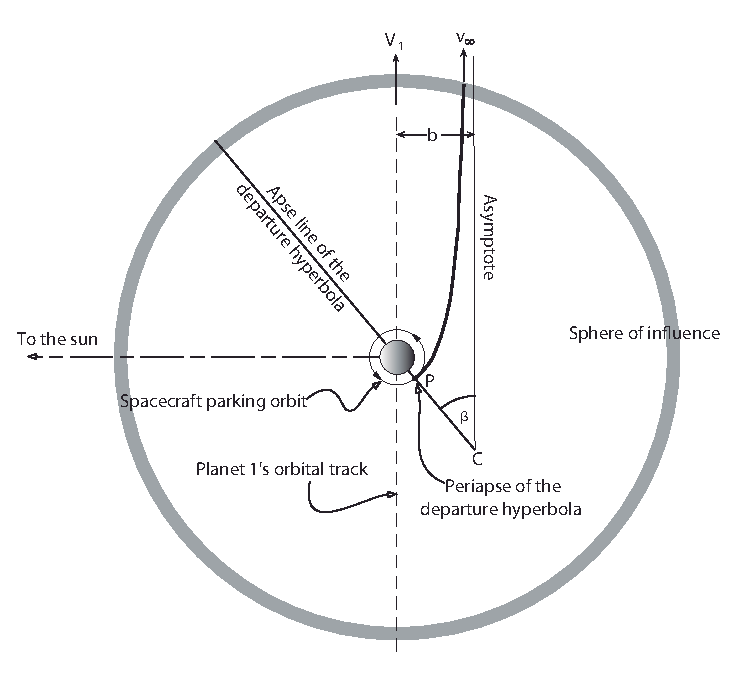
\includegraphics[width=0.5\textwidth]{././images/1stStage1} 
	\caption{Hyperbola Parameters. Extracted from~\cite{llibreVictor}.}
	\label{fig:HyperParam}
\end{figure}

The hyperbola can also be defined by the semi-major axis (\textit{a}) and the eccentricity (\textit{e}). In addition, the $\Delta V$ necessary to inject the probe into the hyperbolic orbit from the parking orbit must be specified.

To obtain these parameters, only the heliocentric departure speed ($v_1$), the velocity of the departure planet ($v_p$) and the parking orbit (in particular, the periapse radius and the speed of the orbit) are needed.


\paragraph{Definition of hyperbola:}
The first step is to obtain the semi-major axis of the hyperbola. This is obtained from the hyperbolic excess velocity as:
\begin{equation}
	a = \frac{\mu}{V_\infty^2}
\end{equation}

where $\mu$ is the standard gravitational parameter ($\mu=GM$) for the sun and the excess velocity is computed as the difference between the probe velocity and the departure planet speed. The eccentricity of hyperbola is defined by:
\begin{equation}
	e=1+(\frac{V_\infty}{V_0})^2
\end{equation}
where $V_0$ refers to the speed of the parking orbit. If this orbit is assumed to be circular with $r_0$ as the periapse, the probe velocity through the parking orbit is given by:
\begin{equation}
	V_0=\sqrt{\mu_0/r_0}
\end{equation}

being $\mu_0$ the standard gravitational parameter of the departure planet. Once the eccentricity is computed, the beta angle is easily obtained as:
\begin{equation}
	\cos \beta = \frac{1}{e}
\end{equation}

Finally, the exit parameter is computed by means of:
\begin{equation}
	b=a\sqrt{e^2-1}
\end{equation}

Obtaining the center of the hyperbola is a little bit more cumbersome. Given the three velocities ($V_\infty$, $v_p$ and $v_1$), the two frames of the figure~\ref{fig:frames} can be defined. One has the Y-axis in the direction of the planet velocity and the other has the vernal point over the X-axis. Then, the angle between the planet velocity and this X-axis is defined as $\lambda_v=90+\lambda_x$. Determining this $\lambda_x$ at the injection time $t_1$ 
allows us to obtain the right ascension ($\alpha$) and the declination ($\delta$) of the $v_1$ velocity by means of a change of frame:
\begin{equation}
	\left[\vec{V_\infty}\right]_\mathcal{Q}=\mathcal{R}_1(-\varepsilon)\mathcal{R}_3(-\lambda_x)	\left[\vec{V_\infty}\right]_\mathcal{K}
\end{equation}
Thus,
\begin{equation}
	\sin \delta =\left[V_z\right]_\mathcal{Q}; \qquad \tan \alpha=\left[\frac{V_y}{V_x}\right]_\mathcal{Q}
\end{equation}
Finally, the center of the hyperbola has the following coordinates ($\alpha+12^h$, $\delta$).
\begin{figure}[H]
	\centering
	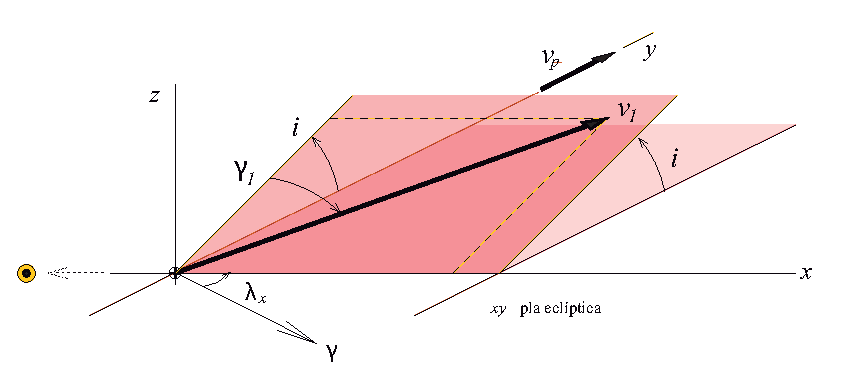
\includegraphics[width=0.5\textwidth]{././images/1stStage2} 
	\caption{Velocities frames of reference. Extracted from~\cite{PCA}}
	\label{fig:frames}
\end{figure}
\paragraph{Delta-v determination}
The necessary delta-v to put the probe onto the hyperbolic departure trajectory is given by:
\begin{equation}
	\Delta V=v_p-V_0=\sqrt{V_\infty+2V_0}-V_0
\end{equation}
The only requirement of the plane of the departure hyperbola is that it must contain the planet center of mass as well as the hyperbolic excess velocity. Therefore, the delta-v has to be applied once the probe flies over C, at a distance of $r_0*\sin \beta$. The circle of all the possible perigees is the injection points circle.
\begin{figure}[H]
	\centering
	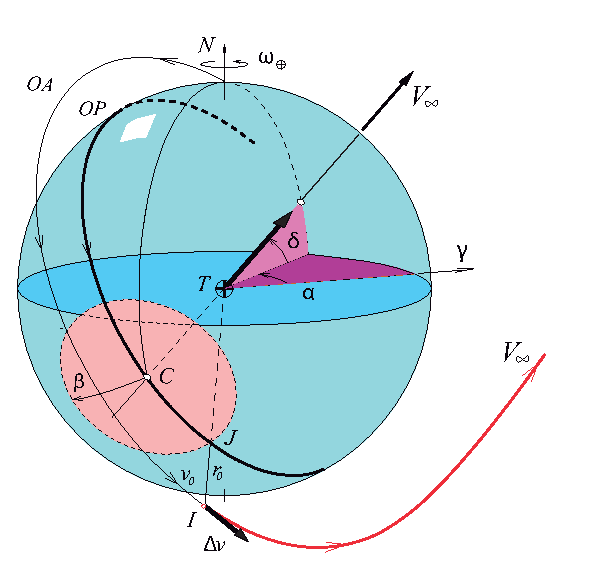
\includegraphics[width=0.5\textwidth]{././images/1stStage3} 
	\caption{Injection points circle. Extracted from~\cite{PCA}}
\end{figure}


